The proposal motivating this project is fundamentally about budgeted reasoning, not merely prefix classification.
For that reason we report decision-quality metrics that remain sensitive to intervention timing and budget allocation.

\paragraph{Budget-conditioned regret.}
The budget-aware artifact shows that the controller ranking changes across domains and across budget bins.
On arithmetic, \directpolicy wins the most budget bins, while \orderedscalar and exact-state factorization each win a substantial minority.
On linear equations, \directpolicy and exact-state factorization dominate the budget bins and \orderedscalar wins none.
This is consistent with the mechanism story:
linear is the domain where scalar thresholding is most visibly mismatched to the action structure.

\paragraph{Revision harm.}
Revision harm is intentionally asymmetric.
A controller is not penalized merely for revising; it is penalized for revising when the oracle says the current prefix should simply continue.
The resulting rates are not globally large, which is useful to know.
But the non-zero harm that remains is concentrated in factorized controllers, especially the deployable predicted-state controller.
That concentration matters because it shows that the remaining structured-controller problem is not ``whether to revise at all'' but ``whether the controller can identify the right time to revise under noisy state estimates''.

\paragraph{Compute-value calibration.}
Calibration turns out to be one of the cleanest diagnostics in the paper.
Exact-state factorization gives the strongest compute-value ordering signal on linear equations.
Predicted-state factorization sharply degrades that ordering in both domains.
Meanwhile, the learned one-dimensional controller often fails to preserve the correct monotone ordering of compute value at all.
This is important because it separates two notions that are often conflated: confidence and value of additional computation.

\begin{figure}[t]
\centering
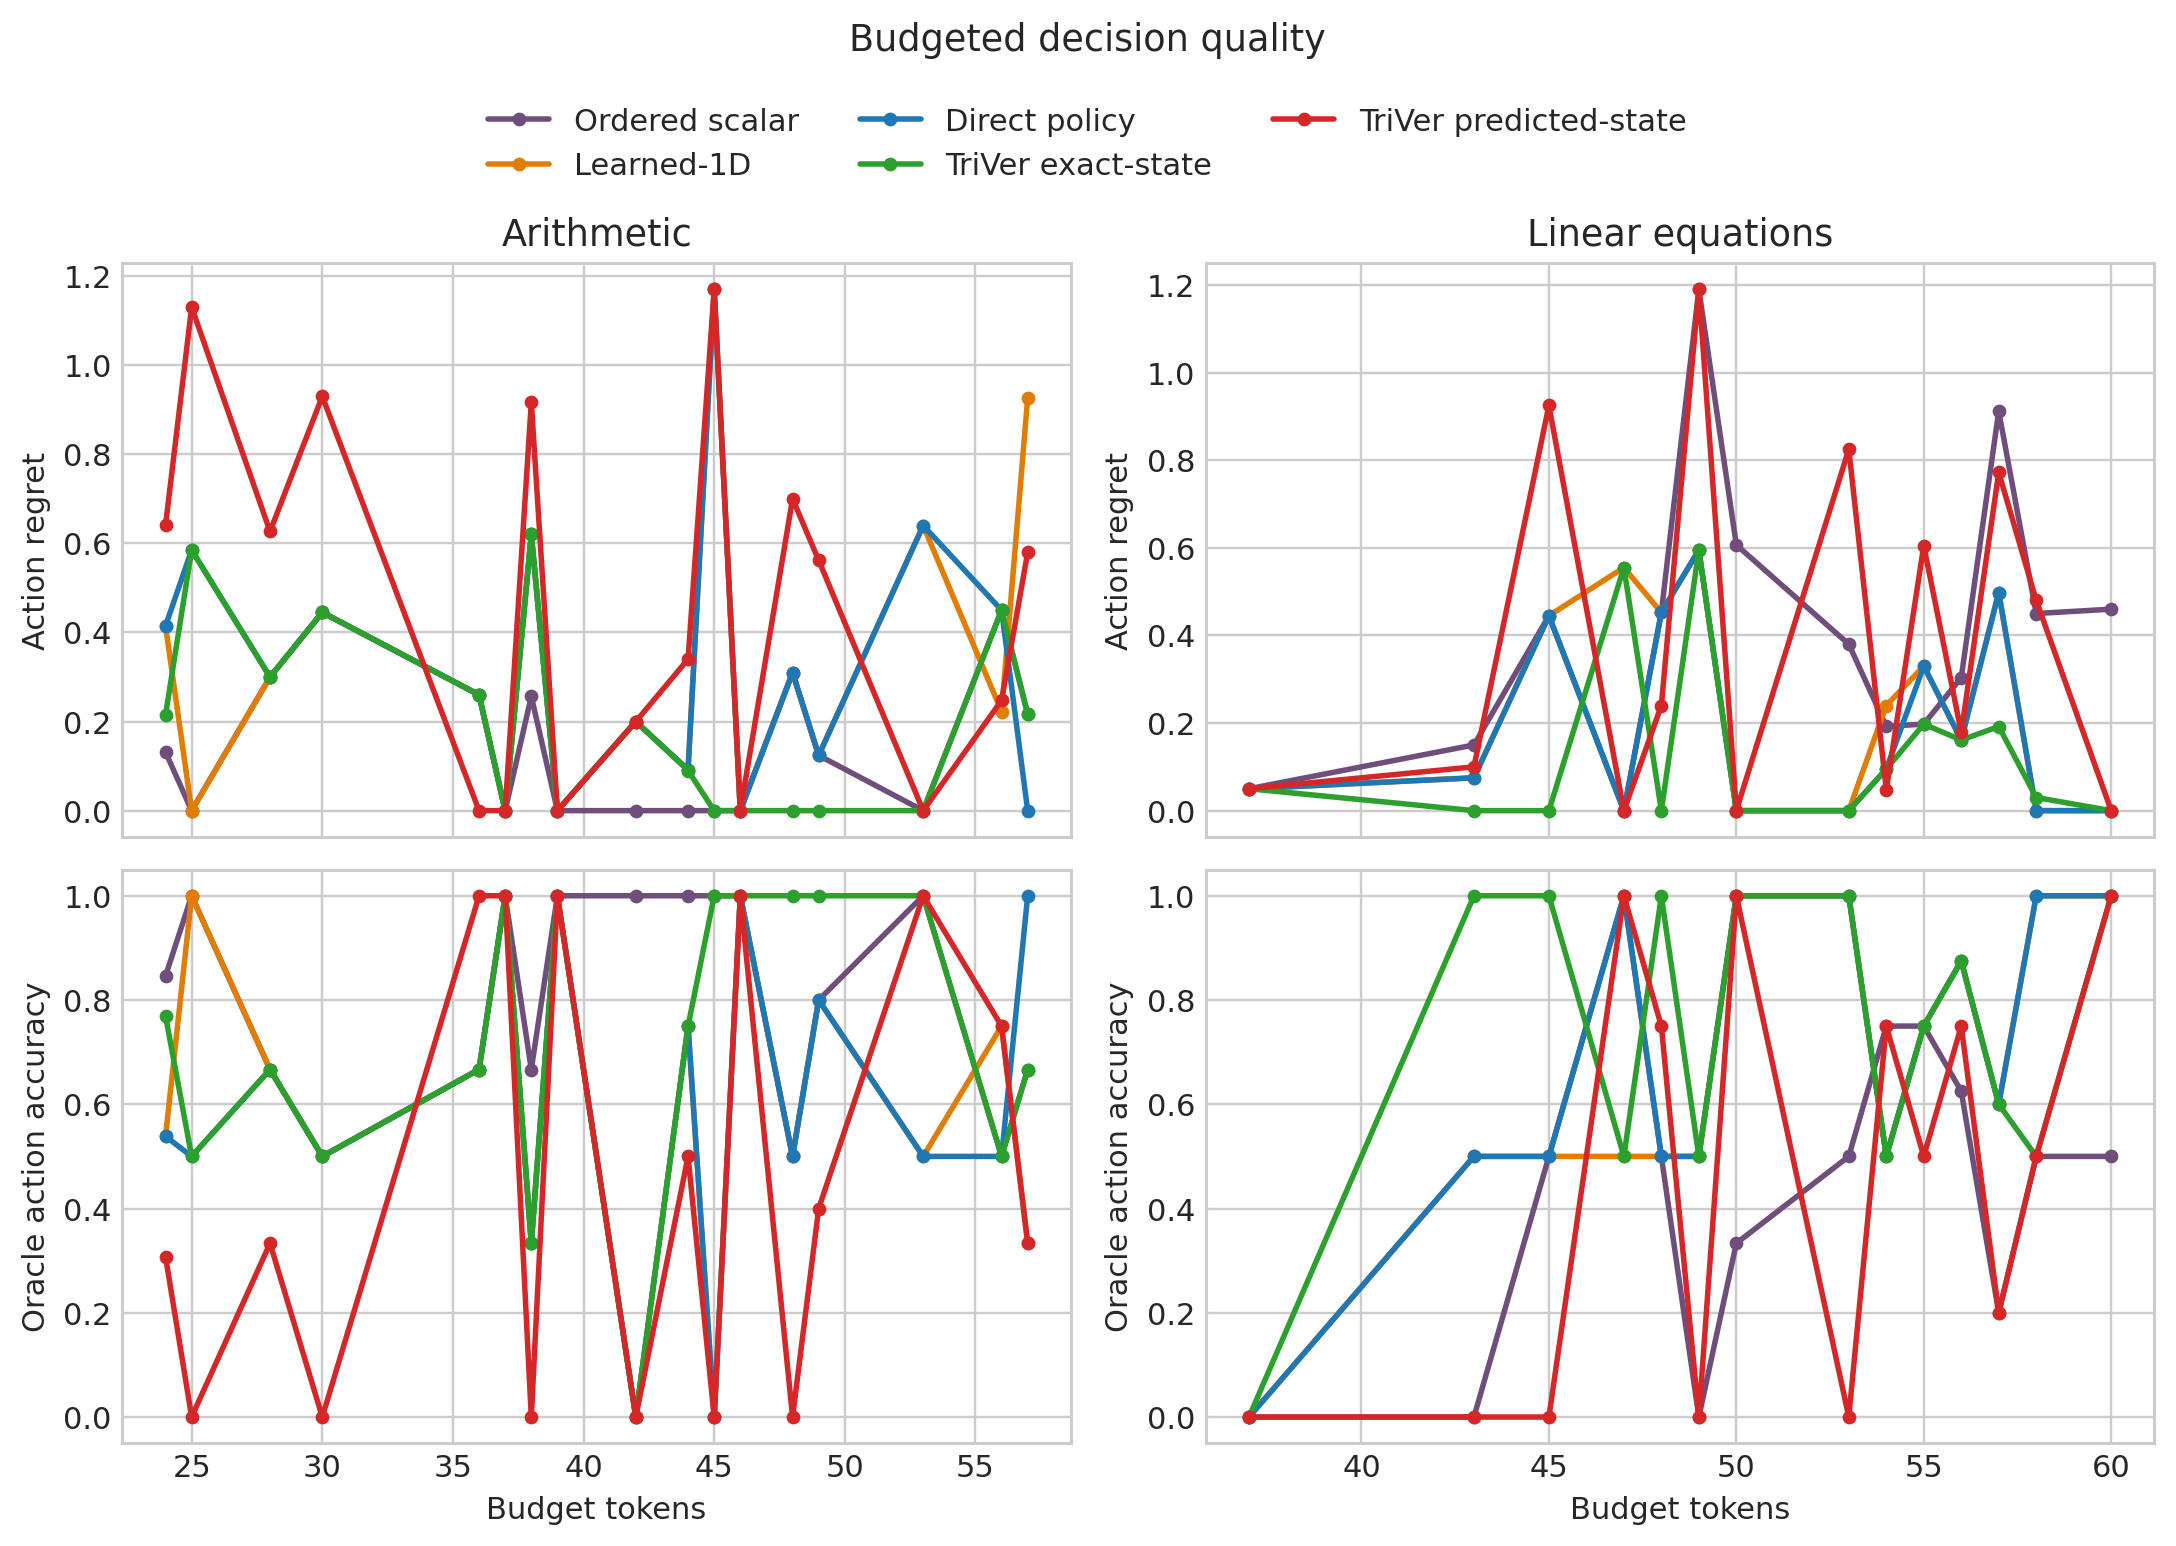
\includegraphics[width=\linewidth]{figures/budget_quality.pdf}
\caption{Budgeted decision quality across domains. The top row reports action regret as a function of budget; the bottom row reports equal-token frontier accuracy at matched token cost. Reading the figure left-to-right shows why the paper is not a pure architecture race: controller rankings move with domain and budget, but predicted-state factorization remains deployment-limited in both domains.}
\label{fig:budget}
\end{figure}

\begin{table*}[t]
\centering
\caption{Budget-aware controller behavior summarized by domain. ``Budget-bin wins'' counts how many budget bins are won by each controller, while ``Calibration'' is the rank correlation between the controller's compute-value proxy and true compute value. The table is meant to summarize decision quality rather than raw leaderboard position: low regret, low revision harm, and good compute-value ordering need not coincide in the same controller.}
\label{tab:budget_wins}
\begin{tabular}{llrrr}
\toprule
Domain & Controller & Budget-bin wins & Revision harm & Calibration \\
\midrule
Arithmetic & \directpolicy & 6 & 0.000 & 0.525 \\
Arithmetic & \orderedscalar & 4 & 0.000 & 0.610 \\
Arithmetic & \triver exact-state & 4 & 0.000 & 0.589 \\
Arithmetic & \triver predicted-state & 1 & 0.019 & -0.031 \\
\midrule
Linear & \directpolicy & 8 & 0.000 & 0.651 \\
Linear & \triver exact-state & 5 & 0.047 & 0.805 \\
Linear & \triver predicted-state & 1 & 0.047 & 0.128 \\
Linear & \orderedscalar & 0 & 0.000 & 0.628 \\
\bottomrule
\end{tabular}
\end{table*}

Table~\ref{tab:budget_wins} turns the budget-dependent story into a concise summary.
The exact-state controller is the most interpretable structured upper bound because it combines low regret with strong calibration.
The predicted-state controller is the most informative deployment diagnostic because it carries both regret and calibration penalties.
The combination of Figures~\ref{fig:gap} and~\ref{fig:budget} is therefore central to the paper's story:
the benchmark is not only exposing controller rankings, but also showing \emph{why} some rankings fail to survive deployment or budget shifts.

These budget-aware results also clarify why the paper should not be framed as a pure architecture race.
The value of the benchmark is precisely that it keeps the decision-quality question visible even when controller rankings move across domains or scales.
